This chapter focuses on describing the set of tools used for this work.

% EXPLAIN  MORE ABOUT THIS CHAPTER


\section{Tools}

This section describes the tools that made this work possible.

\subsection{C++}

C++ is a general purpose programming language that is highly efficient and flexible.
It is greatly focused on performance allowing low-level memory manipulation \cite{C++}.

The ITAndroids Soccer3D base code was already in C++ and therefore, anything that interacts with the soccer simulation server
was also in C++ to integrate seamlessly with the codebase.
For this work, we used version 14 which is the most recent standardized (and stable) version.

\subsection{Python}

Python is an interpreted general purpose high-level programming language \cite{Python}. It has an easy-to-read syntax
closely resembling pseudocode therefore it allows faster development time which makes it easy to prototype new ideas.
For these reasons, the scientific community's usage of Python has greatly increased in recent years, even more so in the
deep learning community. 

For this work, we chose version 3.5 since it is the most recent and stable version when starting development.


\subsection{Protocol Buffers}

Protocol Buffers is a multiplatform library for serializing structured data that supports multiple programming languages \cite{ProtoBuf}.
It is very useful for developing uncoupled client-server applications that communicate using a simple and flexible API.

For these reasons, we chose Protocol Buffer as the client-server API.

\subsection{OpenAI Gym}

OpenAI Gym is a toolkit for running reinforcement learning algorithms in different environments \cite{OpenAIGym}.
It allows testing and benchmarking RL algorithms by providing a standardized set of environments.
This is very important for RL since it makes it accessible for the research community to compare different algorithms \cite{OpenAIGymPaper}.

Figure \ref{fig:openai_env} illustrates a few example environments from OpenAI Gym.

\begin{figure}[H]
    \centering
    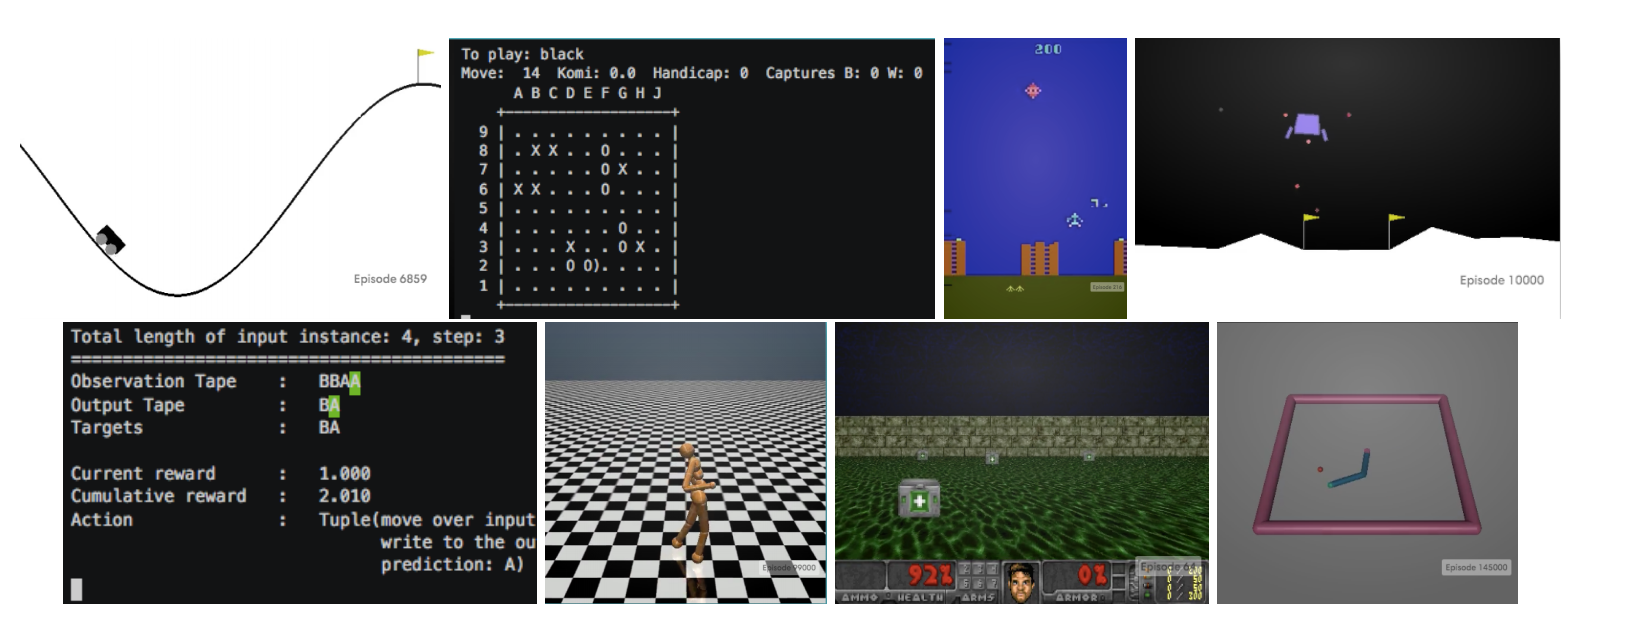
\includegraphics[width=1\textwidth]{Chapter5/openai_env.png}
    \caption{OpenAI Gym environments, extracted from \cite{OpenAIGym}.}
    \label{fig:openai_env}
\end{figure}

Because of these reasons, OpenAI Gym was used in this work.

\subsection{TensorFlow}

TensorFlow is an open source software library for numerical computation using data flow graph \cite{TensorFlow}.
It is greatly used for machine learning applications since it provides efficient implementation of gradient computations and
optimization algorithms that can be parallelized by making use of specialized hardware instructions like SSE and GPU.
The library also exposes an API for multiple languages such as Python, C++, Go and Java.

TensorFlow was chosen because of its big developer community and its various tools available such as Tensorboard, a
visualization dashboard that is very useful for debugging and plotting.

\section{Simulation Environment}

The chosen simulation environment is the \textit{SimSpark} simulator \cite{SimSpark}. 
It is a simulation system for multi-agent simulations and uses Open Dynamics Engine \cite{ODE} for rigid body dynamics and collision detecting.
The system allows two teams of up to eleven humanoid robots to play against each other.

The implementation of SimSpark does not guarantee that events are reproducible and adds noise to the problem.
This makes the problem more challenging to learn, since different instances of the same simulation may have different outcomes.
In addition, it is very important to run the RL algorithms multiple times to reduce the variance in the outcomes.

The server also exposes a network interface that allows external processes to be notified of the simulation's state
for purpose of visualization or logging. This interface allows queries of the ground truth state of 
the simulation state that are not available during regular game play, e.g. the global position of the robot.
The entity that reveals the ground truth is known as the Wizard in the ITAndroids code.

For this work, we used \textit{RoboViz}, a publicly available visualization tool created by Justin Stoecker \cite{RoboViz} that allows a few
improvements over the default visualization tool. Figure \ref{fig:sim3d} shows a typical game scene between two teams inside \textit{RoboViz}.

\begin{figure}[H]
     \centering
     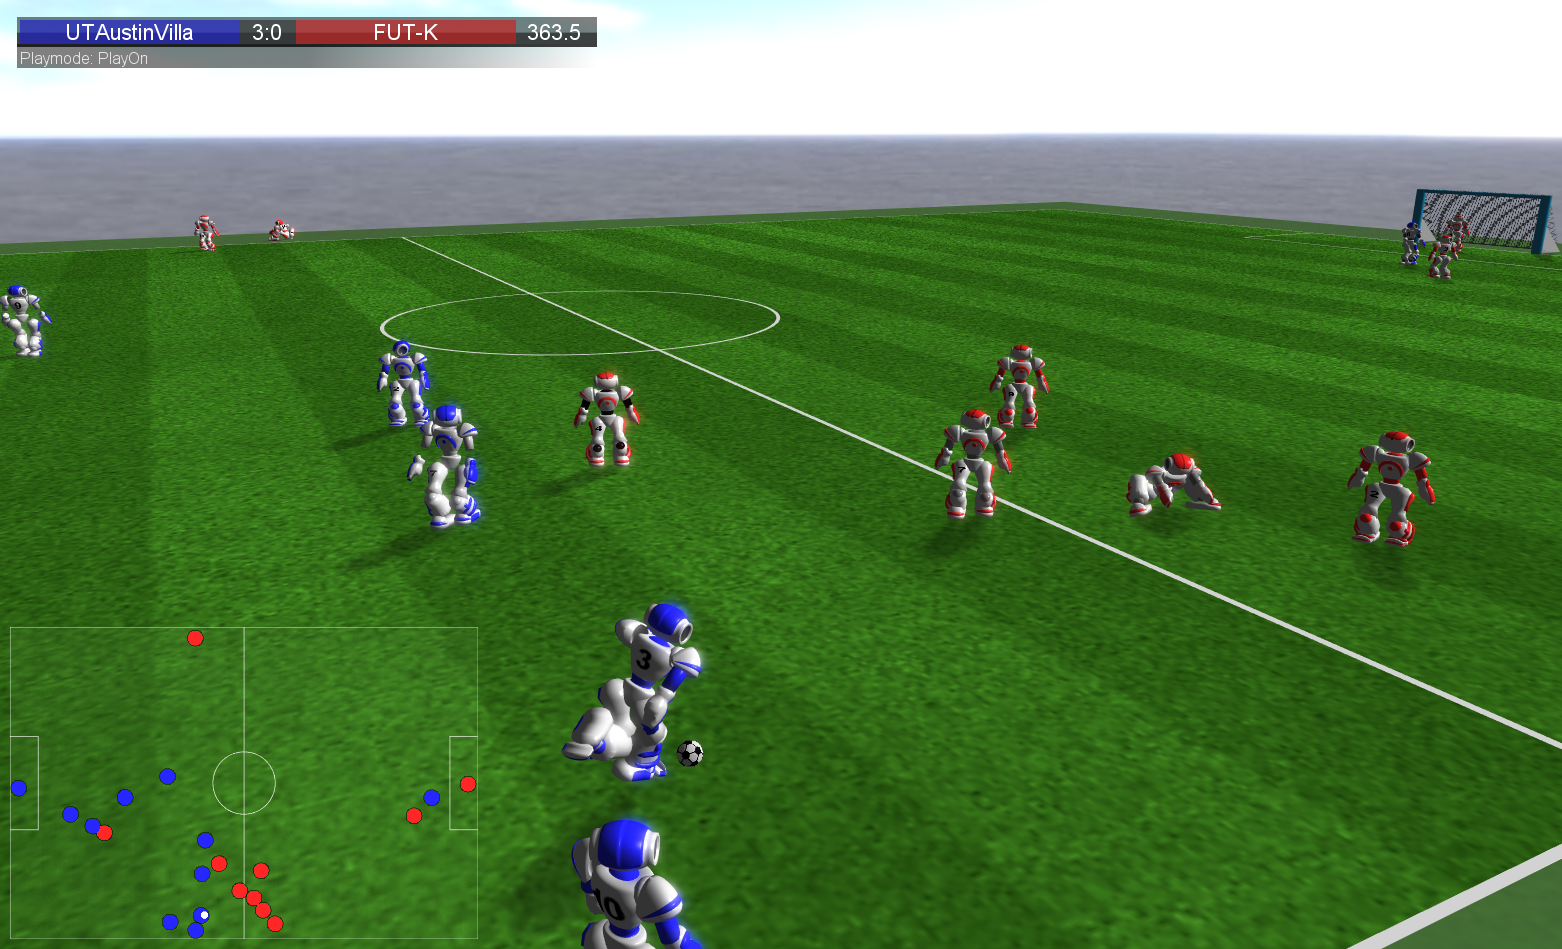
\includegraphics[width=0.95\textwidth]{Chapter5/sim3d.png}
     \caption{\textit{SimSpark} Simulation Environment running.}
     \label{fig:sim3d}
\end{figure}

Agents communicate with the simulator via TCP connections. The agent communicates with the server and the server
executes a simulation step of $\Delta t = 0.020$ s. At each timestep, the robot sends the desired speed values of each joint to the server
and this is how the agents perform actions within the simulation \cite{SimSparkEffectors}.

Our simulated agent is a simulation of the Nao humanoid robot manufactured by SoftBank Robotics \cite{NaoRobot} and has 22 joints (or degrees of freedom).
Therefore, to make the robot act as desired, at each timestep, we must calculate all 22 joint velocities for the robot.
Figure \ref{fig:nao} depicts the real Nao robot.

\begin{figure}[H]
    \centering
    
\includegraphics[width=0.25\textwidth]{Chapter5/nao.png}
    \caption{SoftBank Robotics Nao.}
    \label{fig:nao}
\end{figure}

The main reason this simulation environment was chosen was that it is the official simulator used in RoboCup Soccer Simulation 3D competition since 2004.

\section{Walking Engine}

The omnidirectional walking engine is an algorithm that calculates how the humanoid robot should walk. 
As input, it receives a desired velocity $v = [v_x, x_y, x_{\psi}]^T$ , where $v_x$, $v_y$ and $v_{\psi}$
are speeds in the forward, lateral and rotational directions, respectively and calculates the robot's joint angles as output.
These angles are then fed to PID controllers at each joint to compute the joint velocities actually sent to the server.
A simplified overview of the walking engine is shown in Figure \ref{fig:walkingengine}.
In this work, we are not interested in the walking engine per se, however it is important to understand some low-level aspects
of the walking engine since it implies in some design restrictions on how the robot walks and influences the learned behavior.

A popular concept in the humanoid literature is the Zero Moment Point (ZMP) \cite{ZMP}.
The ZMP can be thought of the dynamic version of the center of mass (CoM) due to the following stability
criterion: a biped is dynamically stable at a given time instant if the ZMP is inside the support polygon
(the convex hull of all contact points on the ground) \cite{ZMP}.
The walking engine we use is based on \cite{MestradoManga, CaminhadaManga}.
The engine is based on the Zero Moment Point (ZMP)
and approximates the robot dynamics using the Linear Inverted Pendulum Model \cite{Kajita}.

The walking engine can be described as the following components:

\begin{itemize}
    \item \textbf{Footstep planner:} decides the torso and swing foot poses of the robot at the end of the step.
    \item \textbf{CoM Trajectory Generator:} determines the trajectory for the CoM in order to achieve these planned poses.
    Essentially, the ZMP must always be within the support polygon during a step and the CoM trajectory must always
    match the CoM positions at the beginning and at the end of the step. This defines a boundary value problem that can
    be solved analytically and the solution describes the trajectory for the CoM.
    \item \textbf{Swing Foot trajectory Generator:} determines the trajectory for the swing foot by interpolating between
    the initial and final poses of the robot's feet. 
    \item \textbf{Inverse Kinematics (IK) Solver:} calculates the joint angles through IK.
\end{itemize}

A simplified overview of the walking engine is shown in Figure \ref{fig:walkingengine}.

\begin{figure}[htb]
    \centering
    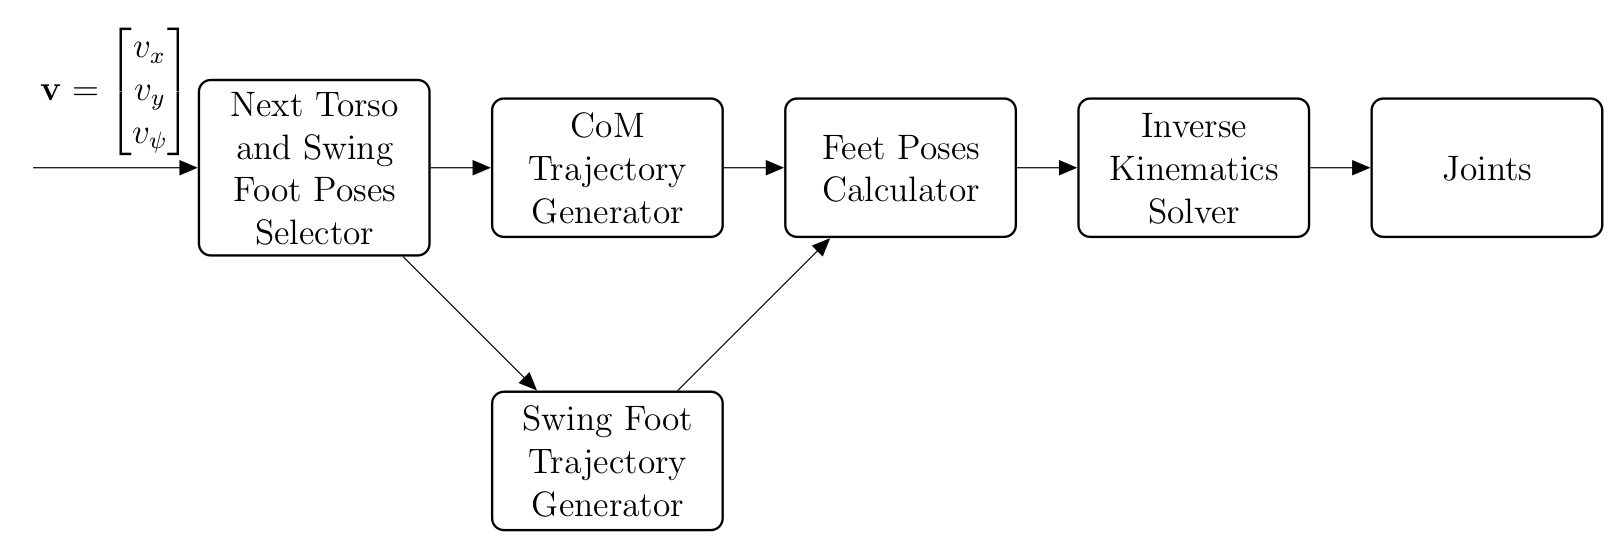
\includegraphics[width=0.95\textwidth]{Chapter5/walkingengine.png}
    \caption{Walking Engine overview.}
    \label{fig:walkingengine}
\end{figure}

The walk cycle, shown in Figure \ref{fig:walk_cycle} has constant duration $T$ and the support foot always alternates between
the right and left, having two double support phases in each step.

\begin{figure}[ht]
    \centering
    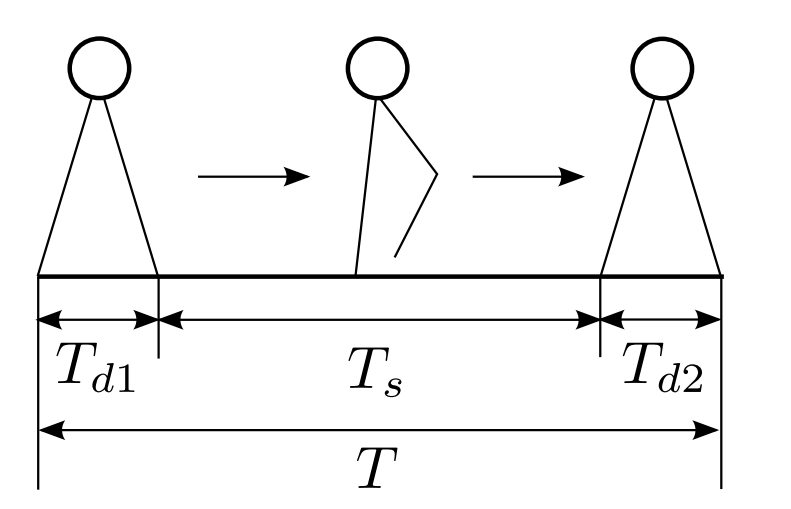
\includegraphics[width=0.7\textwidth]{Chapter5/humanoid_step.png}
    \caption{Walk cycle (a step).}
    \label{fig:walk_cycle}
\end{figure}

Also, for stability purposes, the acceleration is bounded, so it may take multiple walking steps to 
reach the desired speed. For details, please  refer to \citen{MestradoManga}.

\section{Metrics}
\label{sec:metrics}

When trying to solve some reinforcement learning task, it is very important to define a few metrics
that effectively provides information during the training stage. With this information we try to understand
how well the agent is doing in its task.
In this work, we focused on 2 main metrics:

\begin{itemize}
    \item \textbf{Episode accumulated reward:} Maximizing the episode return is the goal of RL therefore
     it is the most obvious performance indicator and gives a very good sense of how well the agent's actions are doing.
    \item \textbf{Episode duration:} Episode reward is the central element in the RL framework to describe how
    well the agent is doing, however, for some further intuition, 
    it is also interesting to observe how long each episodes is taking in time.
    For example, for the \textit{Racing Domain}, if the episode is finishing early, it is a good indicator
    that the robot is falling or leaving the race track early.
    \item \textbf{Data efficiency:} A quantitative measure of how long an agent takes to learn a good behavior.
\end{itemize}

These are the metrics we used for all the tasks however. 
We have also made use of task specific metrics that further try to measure the agent's performance.
These metrics are described in Chapter \ref{chap:contrib}.

All the metrics were calculated in an offline manner, that is, after the simulation finished.
This was possible since we logged all the state and action information from the agent for each episode on the server side
and was very helpful for reviewing past runs to extract non-obvious conclusions from the data.